\section{The object flow estimation pipeline}
\label{sec:desc}

Following the definition of the problem given above we have devised a system for computing the object flow.
The Fig. \ref{figurelabel_sys} shows a simplified block diagram of the proposed system. It is important to recognize the two main 
components of our work-flow: object tracking and segmentation, and pixel-wise flow computation on the pixels of interest.  The scheme is completed by feeding back the flow 
information to improve the tracker as depicted in the figure. For instance, one can make the most of dense displacement vectors to refine the motion of the target, and 
the segmentation information can be used to improve the sampling process of the learning stage in several trackers by detection methods \cite{c22}. Thus, 
the tracker and motion flow algorithm can work for mutual enhancement.

\ifcsdef{r@accv_format}{

   \begin{figure}[thpb]
      \centering
      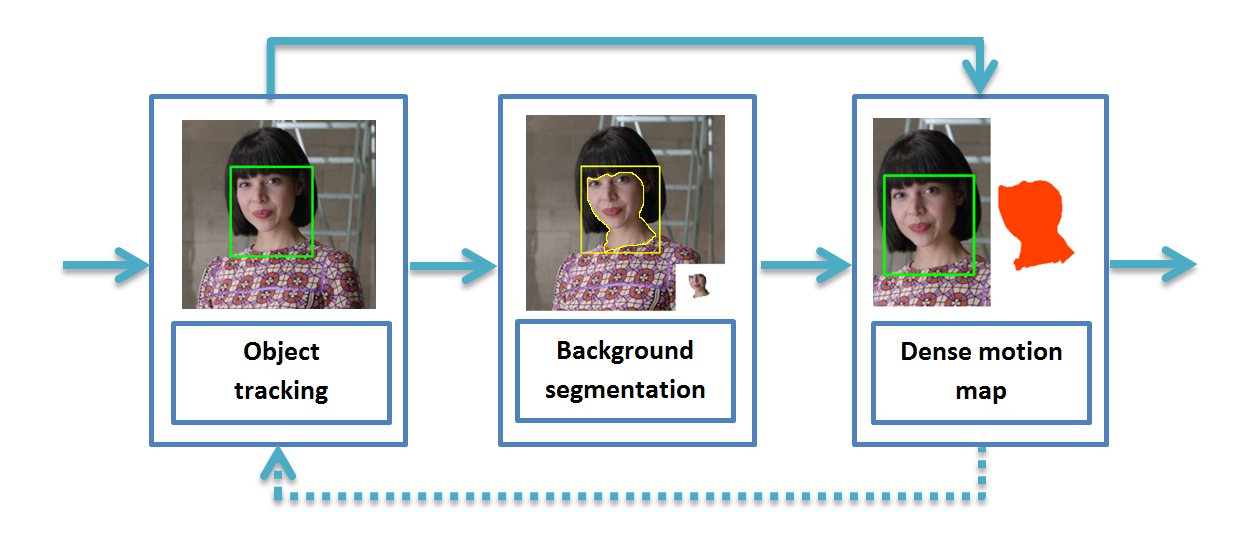
\includegraphics[width=1.00\textwidth]{../images/system.png}
      \caption{Block diagram of the object flow pipeline.}
      \label{figurelabel_sys}
   \end{figure}
}{
   \begin{figure}[thpb]
      \centering
      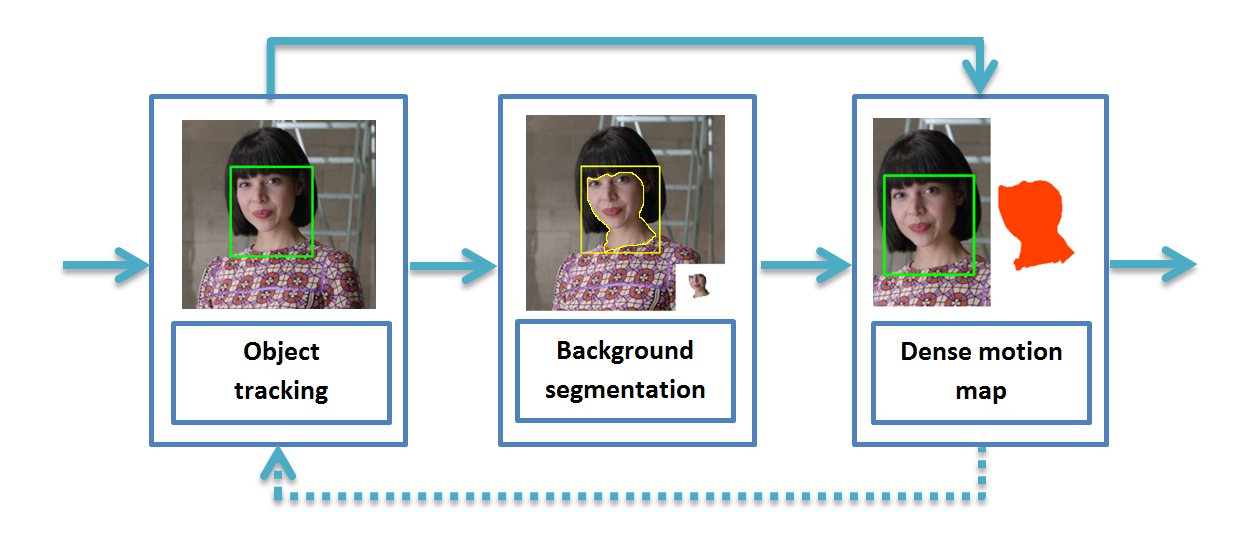
\includegraphics[width=0.5\textwidth]{../images/system.png}
      \caption{Block diagram of the object flow pipeline.}
      \label{figurelabel_sys}
   \end{figure}
}

Object tracking in the object flow pipeline can be selected according to a specific need for a given application. Here we prefer recent methods based on tracking-by-detection given 
that they are in the top of modern benchmarks for object tracking \cite{c16} in terms of accuracy and stability to initialization changes.

